\subsection{Definition des Modells}
\label{sec:ModellDefinition}
Ziel dieses Unterabschnitts ist es herauszuarbeiten, wie mehrere ConvLSTM-Layer zusammen mit anderen Layertypen für räumlich-zeitliche Vorhersagen verwendet werden können.
Außerdem wird eine Verlustfunktion definiert, die für den vorliegenden Anwendungsfall geeignet ist.

ConvLSTM-Layer können unterschiedlich verwendet werden, um bestimmte Anwendungsfälle abzudecken.
Die wichtigste Unterscheidung ist, ob die Ausgabe des Modells eine Sequenz oder ein einzelner 2D-Tensor sein soll.
Der erste Fall wird beispielsweise für die Weiterführung einer Bildsequenz verwendet, wie in \cite{VideoPredKeras} demonstriert.
Eine solche Architektur könnte im Kontext der vorliegenden Arbeit beispielsweise verwendet werden, um die Gefahr für mobile Radarkontrollen mehrere Tage vorauszusagen.
Dies ist jedoch hier nicht notwendig.
Eine alternative Architektur wird in \cite{CrimeConvLSTM} vorgestellt.
Diese ist dazu in der Lage, anhand einer Sequenz von 16 oder 32 2D-Eingangstensoren den folgenden 2D-Tensor vorherzusagen.
Die Architektur wurde im Kontext der Verbrechensvorhersage entwickelt.
Da es sich dabei ebenfalls um sporadisch auftretende Ereignisse handelt, ist die Architektur mit hoher Wahrscheinlichkeit auch für den vorliegenden Anwendungsfall geeignet.
Die Architektur ist in \autoref{fig:ArchCrimeConvLSTM} dargestellt.

\begin{figure}[ht!]
    \centering
    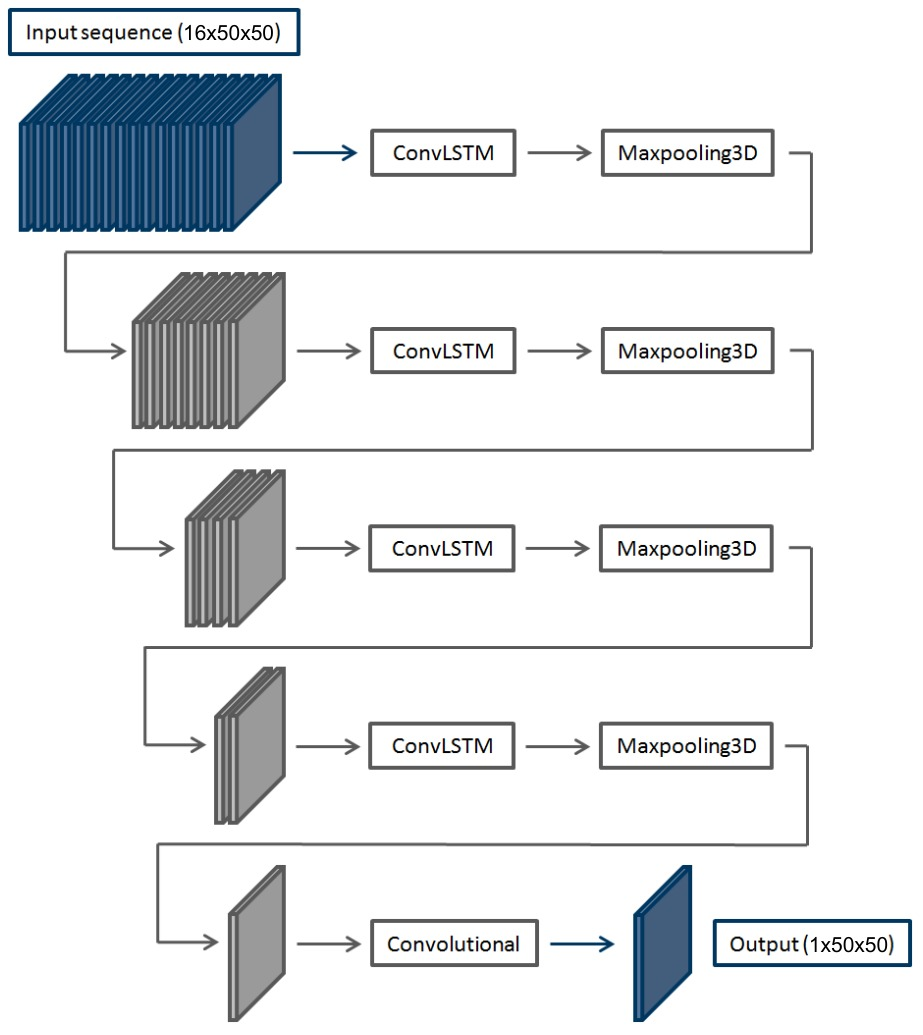
\includegraphics[width=1.0\textwidth,height=16cm,keepaspectratio=true]{content/images/ArchCrimeConvLSTM.jpeg}
    \caption{Architektur eines Modells aus mehreren ConvLSTM- und MaxPooling-Layern nach \cite[Figure 2.1]{CrimeConvLSTM} mit angepassten Dimensionen}
    \label{fig:ArchCrimeConvLSTM}
\end{figure}

Anhand der Abbildung kann der Datenfluss verfolgt werden.
Wie ganz oben zu erkennen ist, hat die Eingabesequenz eine Größe von 16x50x50.
Die Eingabe ist also eine Sequenz von 16 Frames, die jeweils 50x50 Pixel groß sind.
Es ist anzumerken, dass die Eingabesequenz in \cite{CrimeConvLSTM} die Dimensionen 50x50x16 hat.
Die erste und letzte Dimension ist für die vorliegende Arbeit getauscht, da die Verarbeitung so intuitiver ist.
Das Resultat ist jedoch dasselbe.
Die Eingabe durchläuft nun mehrmals je einen ConvLSTM- und einen MaxPooling3D-Layer.
Die ConvLSTM-Layer haben nach \cite{CrimeConvLSTM} eine Kernelgröße von 3x3 Pixel.
Außerdem werden Höhe und Breite der Frames durch Padding beibehalten.
Auch die Anzahl an Frames bleiben durch die ConvLSTM-Layer erhalten.
Um von den 16 Frames auf ein Frame als Ausgang zu kommen, befindet sich hinter jedem ConvLSTM-Layer ein MaxPooling3D-Layer.
Dieser Layer berechnet je das Maximum zweier Pixel, die in zwei benachbarten Frames an derselben Position liegen.
Dies entspricht einer Poolgröße von $(2, 1, 1)$.
Außerdem wird eine Schrittweite von $(2, 1, 1)$ verwendet.
Das Resultat ist (vereinfacht auf 3x3 Pixel) in \autoref{fig:MaxPooling3D} dargestellt.

\begin{figure}[ht!]
    \centering
    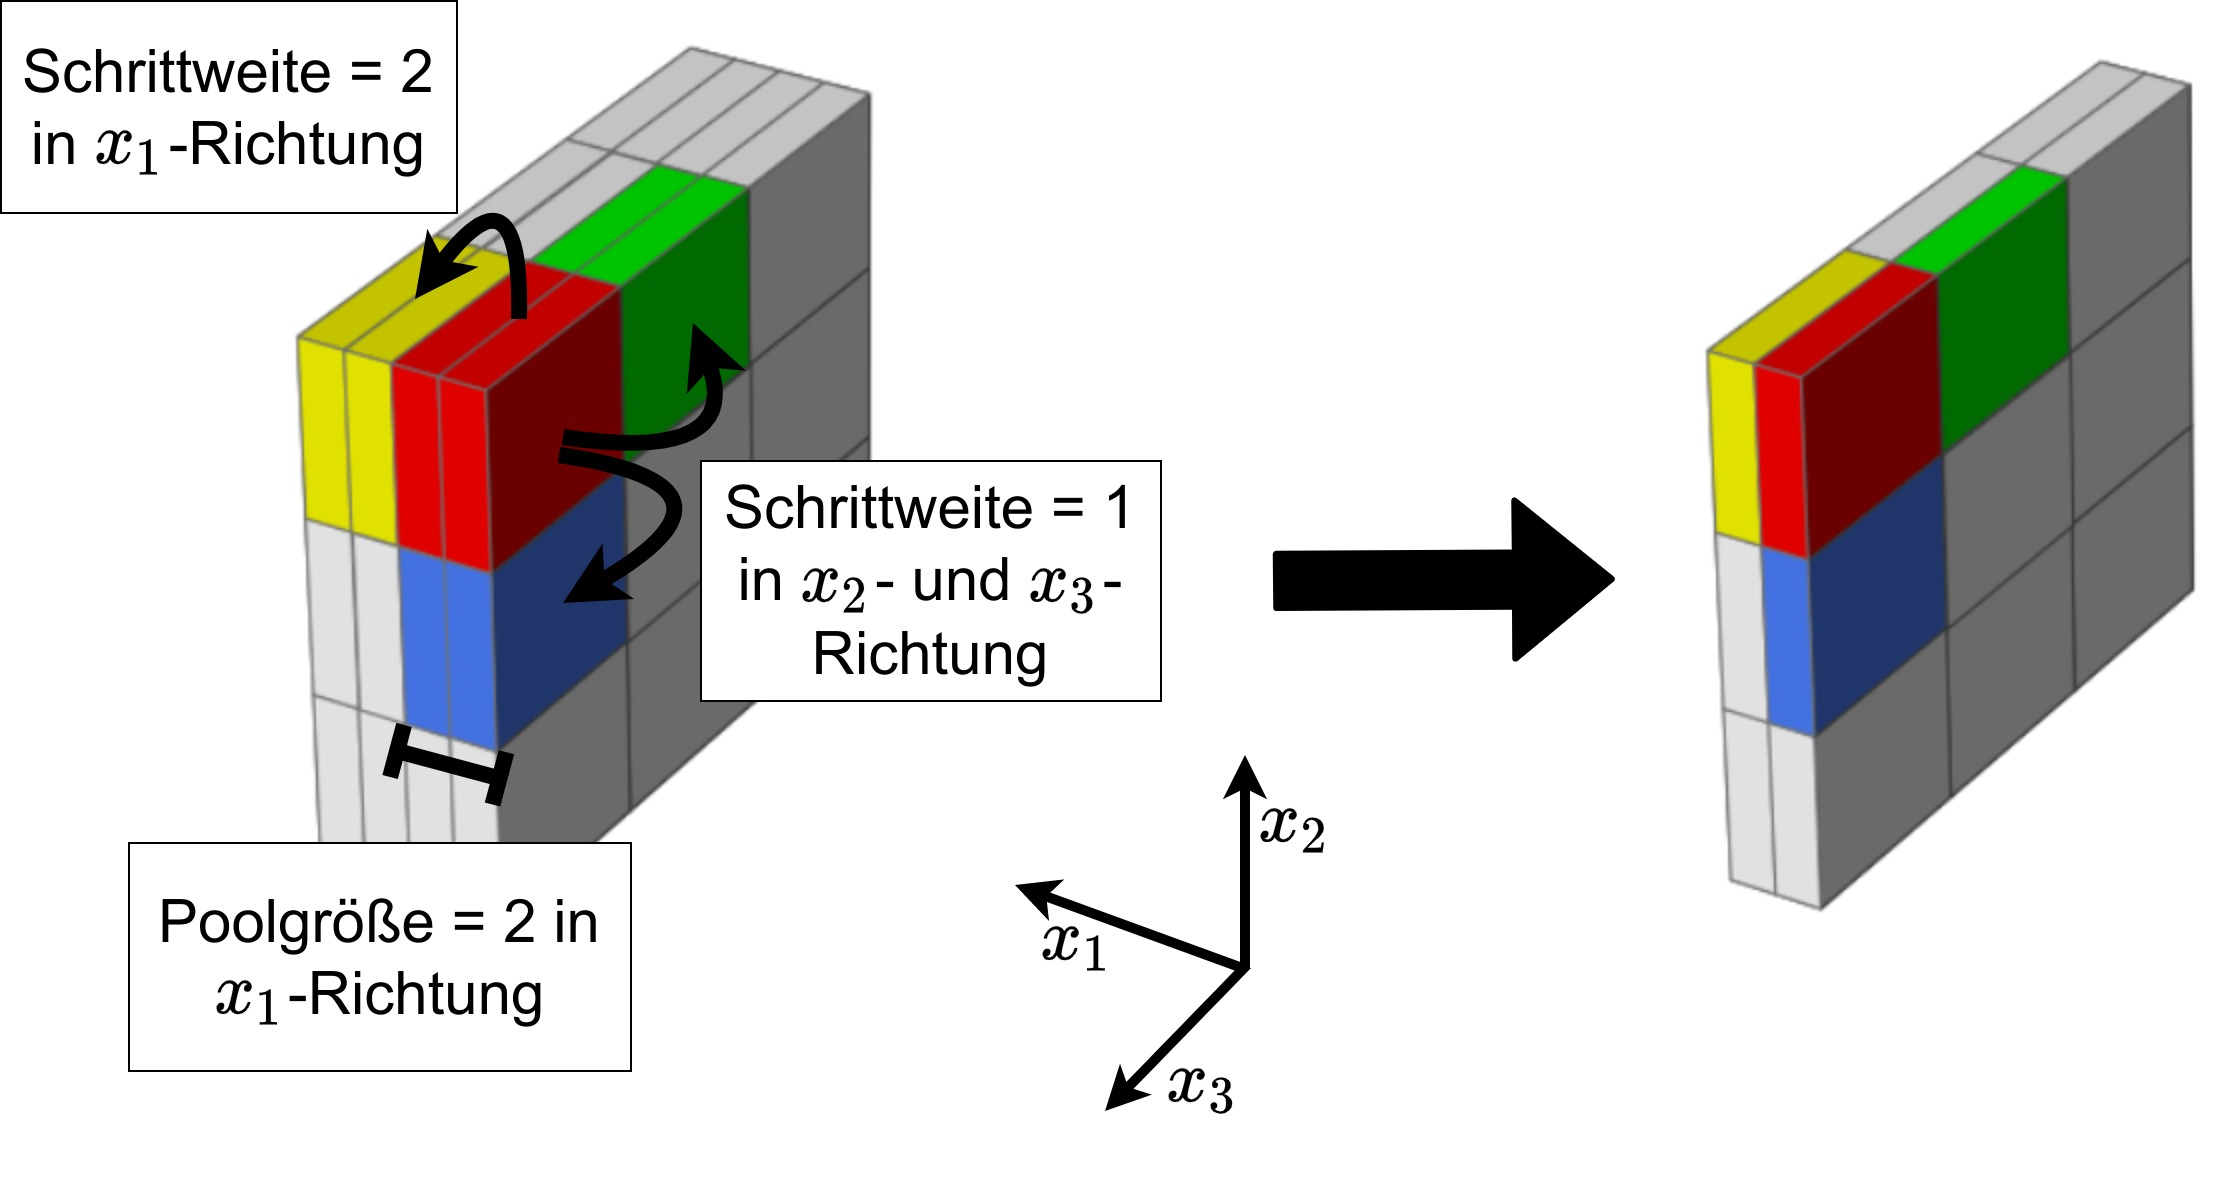
\includegraphics[width=0.8\textwidth,height=8cm,keepaspectratio=true]{content/images/MaxPooling3D.jpeg}
    \caption{Visualisierung der MaxPooling3D-Operation mit einer Poolgröße von $(2, 1, 1)$ und einer Schrittweite von $(2, 1, 1)$ anhand von vier Eingangsframes zu je 3x3 Pixeln}
    \label{fig:MaxPooling3D}
\end{figure}

Mit der MaxPooling3D-Operation werden damit die signifikantesten Merkmale von je zwei benachbarten Frames vereint.
Dadurch wird die Anzahl der Frames in der Sequenz nach jeder ConvLSTM-MaxPooling3D-Kombination halbiert.
Somit ist nach vier dieser Kombinationen nur noch ein Frame übrig.
Am Ende liegt nach \cite{CrimeConvLSTM} noch ein 3D-Faltungslayer mit einer Kernelgröße von $(1, 3, 3)$.
Dort ist die dreidimensionale Version eines Faltungslayers nötig, da die erste und letzte Dimension wie oben angemerkt vertauscht ist.
Da ein 3D-Faltungslayer mit einer Kernelgröße von $(3, 3, 1)$ (wie er hier verwendet werden müsste) exakt einem 2D-Faltungslayer mit einer Kernelgröße von $(3, 3)$ entspricht, wird hier letzterer verwendet.
% TODO: Zum Abschluss bringen, evtl. Codelisting-Verweis

Um das Modell trainieren zu können muss noch eine Verlustfunktion ausgewählt werden.
Dafür könnte eine gewöhnliche Verlustfunktion für die Klassifizierung wie die binäre Kreuzentropie (engl. \emph{binary cross entropy}) verwendet werden.
Das liegt daran, dass der vorliegende Anwendungsfall als Binärklassifizierung angesehen werden kann: entweder es befindet sich eine Radarkontrolle in einer Rasterzelle oder nicht.
Bei einem ausgeglichenen Datensatz könnte eine solche Verlustfunktion direkt verwendet werden.
Für den vorliegenden Anwendungsfall ist jedoch die Besonderheit zu beachten, dass es in den Daten deutlich mehr Rasterzellen ohne eine einzige Radarkontrolle gibt als Rasterzellen, in denen es mindestens eine gibt.
Mit einer normalen Verlustfunktion werden falsch-negative Ergebnisse genauso hart bestraft wie falsch-positive.
Andersherum werden richtig-positive Ergebnisse genauso begünstigt wie richtig-negative.
Hier ergibt sich jedoch ein Problem.
Ein bei der Trainierung sehr schnell zu findendes Minimum der Verlustfunktion liegt genau dort, wo die Vorhersage des gesamten Rasters "`negativ"' ist.
Somit kann beispielsweise bei einer Positivenrate von 5\% im Datensatz eine Genauigkeit (engl. \emph{accuracy}) von 95\% erzielt werden, wenn alle Rasterzellen als "`negativ"' vorhergesagt werden.
Allerdings entsteht damit keinerlei Erkenntnisgewinn.
Damit der Optimierungsalgorithmus nicht nach kurzer Zeit in dieses schnell zu erreichende Minimum fällt, kann nach \cite{CrimeConvLSTM} eine gewichtete Verlustfunktion verwendet werden.
Eine gewichtete Verlustfunktion weist den einzelnen Klassen Gewichtungen zu, die mit den Kreuzentropiewerten der jeweiligen Klasse multipliziert werden.
Ist die Gewichtung größer als $1$, wird der Wert der Kreuzentropie verstärkt bzw. mehr gewichtet und umgekehrt.
Die in der vorliegenden Arbeit verwendete Verlustfunktion ist in \autoref{lst:WeightedCrossEntropy} dargestellt.

\begin{code}
\begin{minted}[
    linenos,
    numbersep=10pt,
    gobble=0,
    frame=lines,
    framesep=2mm]{python}
def weighted_binary_crossentropy(weights: dict):
    def loss_fn(y_true, y_pred):
        tf_y_true = tf.cast(y_true, dtype=y_pred.dtype)
        tf_y_pred = tf.cast(y_pred, dtype=y_pred.dtype)

        weights_v = tf.where(tf.equal(tf_y_true, 1), weights[1], weights[0])
        crossentropy = K.binary_crossentropy(tf_y_true, tf_y_pred)
        weighted_crossentropy = tf.multiply(crossentropy, weights_v)

        loss = K.mean(weighted_crossentropy)
        return loss

    return loss_fn
\end{minted}
\captionof{listing}{Implementierung einer gewichteten Kreuzentropie als Verlustfunktion für spärliche Daten}
\label{lst:WeightedCrossEntropy}
\end{code}

In Zeile 6 wird die Matrix \emph{weights\_v} berechnet, die die Gewichtungen jeweils an den Stellen enthalten, an denen die jeweilige Klasse in den wahren Daten vorkommen.
In Zeile 7 wird die gewöhnliche binäre Kreuzentropie berechnet.
In Zeile 8 werden dann die Gewichtungen durch elementweise Multiplikation zu den Vorkommnissen der jeweiligen Klasse multipliziert.
Die Matrix \emph{weighted\_crossentropy} enthält nun die gewichtete Kreuzentropie für jeden Datenpunkt, also jede Rasterzelle.
Der Verlustwert berechnet sich dann in Zeile 10 aus dem Durchschnitt aller dieser Werte.

Mit der Netzarchitektur und der Verlustfunktion sind nun alle Bestandteile des Modells definiert.
Daher kann in den folgenden Abschnitten mit der Implementierung begonnen werden.
